\documentclass[14pt]{extbook}
\usepackage{multicol, enumerate, enumitem, hyperref, color, soul, setspace, parskip, fancyhdr} %General Packages
\usepackage{amssymb, amsthm, amsmath, latexsym, units, mathtools} %Math Packages
\everymath{\displaystyle} %All math in Display Style
% Packages with additional options
\usepackage[headsep=0.5cm,headheight=12pt, left=1 in,right= 1 in,top= 1 in,bottom= 1 in]{geometry}
\usepackage[usenames,dvipsnames]{xcolor}
\usepackage{dashrule}  % Package to use the command below to create lines between items
\newcommand{\litem}[1]{\item#1\hspace*{-1cm}\rule{\textwidth}{0.4pt}}
\pagestyle{fancy}
\lhead{Makeup Progress Quiz 2}
\chead{}
\rhead{Version B}
\lfoot{5763-3522}
\cfoot{}
\rfoot{Spring 2021}
\begin{document}

\begin{enumerate}
\litem{
Solve the rational equation below. Then, choose the interval(s) that the solution(s) belongs to.\[ \frac{-7}{7x -4} + -3 = \frac{9}{14x -8} \]\begin{enumerate}[label=\Alph*.]
\item \( x \in [0.02,1.02] \)
\item \( x_1 \in [-0.42, -0.08] \text{ and } x_2 \in [0.02,2.02] \)
\item \( x \in [-1.44,-0.83] \)
\item \( \text{All solutions lead to invalid or complex values in the equation.} \)
\item \( x_1 \in [-1.44, -0.83] \text{ and } x_2 \in [0.02,2.02] \)

\end{enumerate} }
\litem{
Determine the domain of the function below.\[ f(x) = \frac{4}{36x^{2} +54 x + 20} \]\begin{enumerate}[label=\Alph*.]
\item \( \text{All Real numbers except } x = a, \text{ where } a \in [-30.46, -29.67] \)
\item \( \text{All Real numbers except } x = a, \text{ where } a \in [-0.86, -0.7] \)
\item \( \text{All Real numbers except } x = a \text{ and } x = b, \text{ where } a \in [-0.86, -0.7] \text{ and } b \in [-0.74, -0.41] \)
\item \( \text{All Real numbers.} \)
\item \( \text{All Real numbers except } x = a \text{ and } x = b, \text{ where } a \in [-30.46, -29.67] \text{ and } b \in [-24.38, -23.98] \)

\end{enumerate} }
\litem{
Choose the equation of the function graphed below.
\begin{center}
    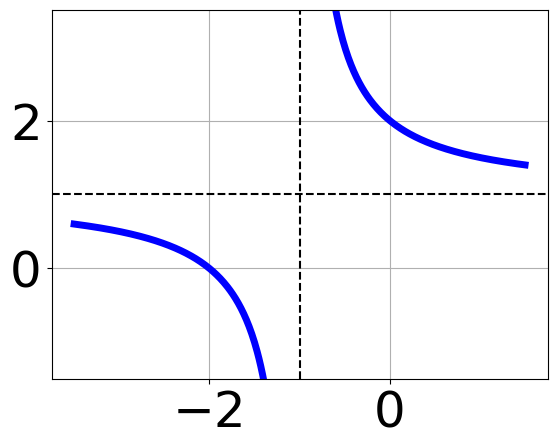
\includegraphics[width=0.5\textwidth]{../Figures/rationalGraphToEquationCopyB.png}
\end{center}
\begin{enumerate}[label=\Alph*.]
\item \( f(x) = \frac{1}{(x + 1)^2} + 6 \)
\item \( f(x) = \frac{-1}{x - 1} + 6 \)
\item \( f(x) = \frac{1}{x + 1} + 6 \)
\item \( f(x) = \frac{-1}{(x - 1)^2} + 6 \)
\item \( \text{None of the above} \)

\end{enumerate} }
\litem{
Choose the equation of the function graphed below.
\begin{center}
    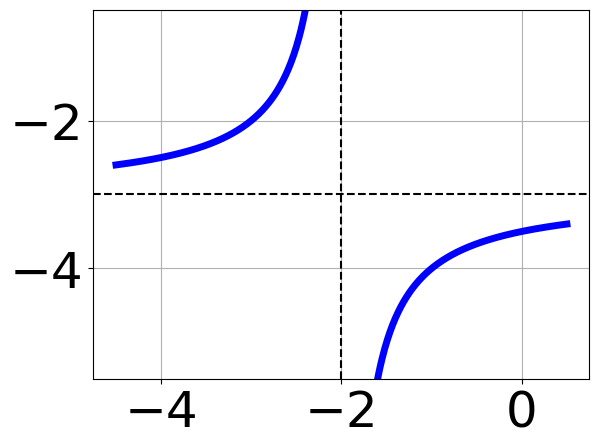
\includegraphics[width=0.5\textwidth]{../Figures/rationalGraphToEquationB.png}
\end{center}
\begin{enumerate}[label=\Alph*.]
\item \( f(x) = \frac{-1}{(x + 2)^2} - 3 \)
\item \( f(x) = \frac{-1}{x + 2} - 3 \)
\item \( f(x) = \frac{1}{x - 2} - 3 \)
\item \( f(x) = \frac{1}{(x - 2)^2} - 3 \)
\item \( \text{None of the above} \)

\end{enumerate} }
\litem{
Solve the rational equation below. Then, choose the interval(s) that the solution(s) belongs to.\[ \frac{-2x}{4x + 6} + \frac{-4x^{2}}{8x^{2} +28 x + 24} = \frac{-5}{2x + 4} \]\begin{enumerate}[label=\Alph*.]
\item \( \text{All solutions lead to invalid or complex values in the equation.} \)
\item \( x_1 \in [-1.42, -0.95] \text{ and } x_2 \in [-5.5,2.5] \)
\item \( x_1 \in [-1.42, -0.95] \text{ and } x_2 \in [-1.17,9.83] \)
\item \( x \in [-2.03,-1.7] \)
\item \( x \in [2.73,3.17] \)

\end{enumerate} }
\litem{
Solve the rational equation below. Then, choose the interval(s) that the solution(s) belongs to.\[ \frac{-25}{35x -45} + 1 = \frac{-25}{35x -45} \]\begin{enumerate}[label=\Alph*.]
\item \( x_1 \in [-1.29, -0.29] \text{ and } x_2 \in [-0.71,2.29] \)
\item \( \text{All solutions lead to invalid or complex values in the equation.} \)
\item \( x \in [1.29,3.29] \)
\item \( x_1 \in [-0.71, 3.29] \text{ and } x_2 \in [-0.71,2.29] \)
\item \( x \in [-1.29,-0.29] \)

\end{enumerate} }
\litem{
Determine the domain of the function below.\[ f(x) = \frac{4}{36x^{2} +42 x + 12} \]\begin{enumerate}[label=\Alph*.]
\item \( \text{All Real numbers except } x = a, \text{ where } a \in [-24.32, -23.59] \)
\item \( \text{All Real numbers.} \)
\item \( \text{All Real numbers except } x = a, \text{ where } a \in [-1.24, -0.57] \)
\item \( \text{All Real numbers except } x = a \text{ and } x = b, \text{ where } a \in [-1.24, -0.57] \text{ and } b \in [-0.52, -0.08] \)
\item \( \text{All Real numbers except } x = a \text{ and } x = b, \text{ where } a \in [-24.32, -23.59] \text{ and } b \in [-18.32, -17.62] \)

\end{enumerate} }
\litem{
Choose the graph of the equation below.\[ f(x) = \frac{-1}{(x - 2)^2} + 1 \]\begin{enumerate}[label=\Alph*.]
\begin{multicols}{2}\item 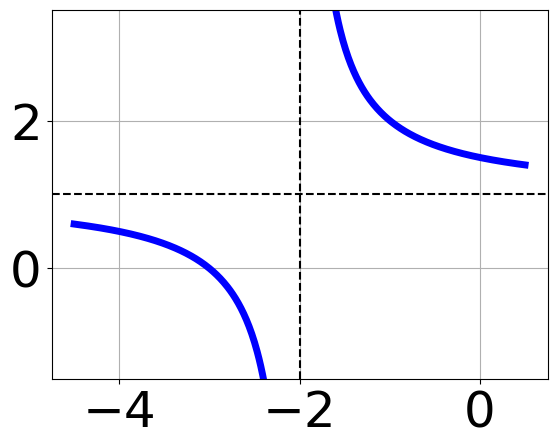
\includegraphics[width = 0.3\textwidth]{../Figures/rationalEquationToGraphCopyAB.png}\item 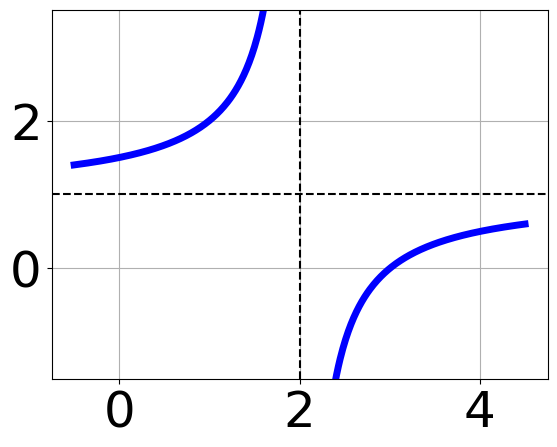
\includegraphics[width = 0.3\textwidth]{../Figures/rationalEquationToGraphCopyBB.png}\item 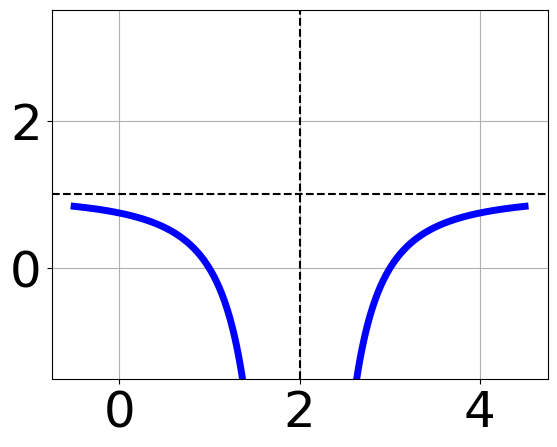
\includegraphics[width = 0.3\textwidth]{../Figures/rationalEquationToGraphCopyCB.png}\item 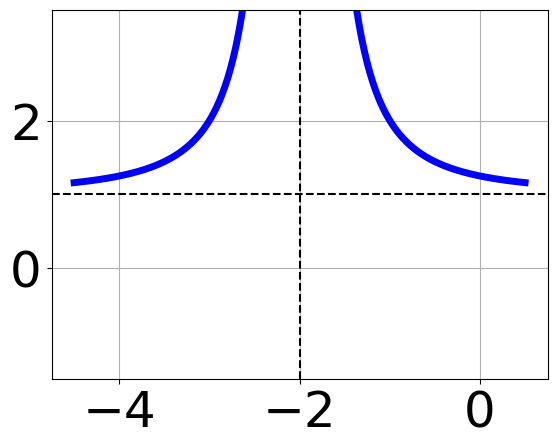
\includegraphics[width = 0.3\textwidth]{../Figures/rationalEquationToGraphCopyDB.png}\end{multicols}\item None of the above.
\end{enumerate} }
\litem{
Choose the graph of the equation below.\[ f(x) = \frac{1}{(x - 3)^2} + 1 \]\begin{enumerate}[label=\Alph*.]
\begin{multicols}{2}\item 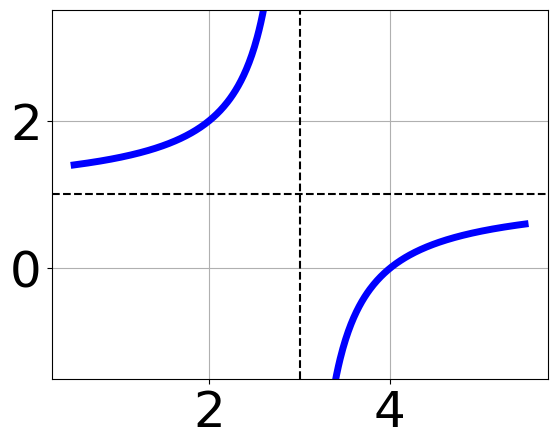
\includegraphics[width = 0.3\textwidth]{../Figures/rationalEquationToGraphAB.png}\item 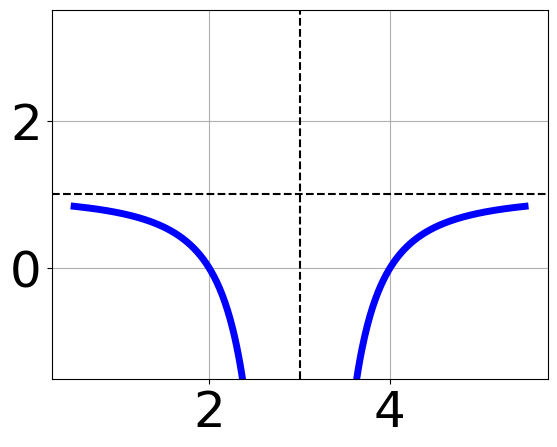
\includegraphics[width = 0.3\textwidth]{../Figures/rationalEquationToGraphBB.png}\item 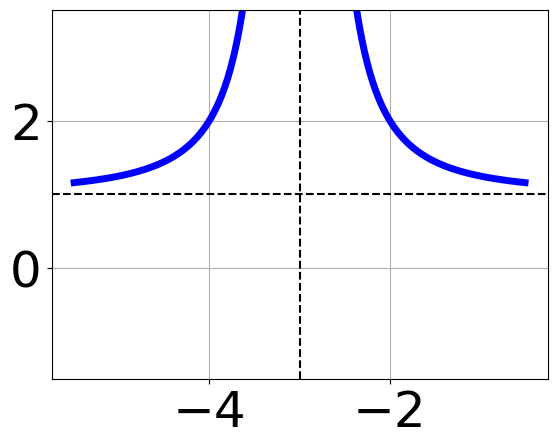
\includegraphics[width = 0.3\textwidth]{../Figures/rationalEquationToGraphCB.png}\item 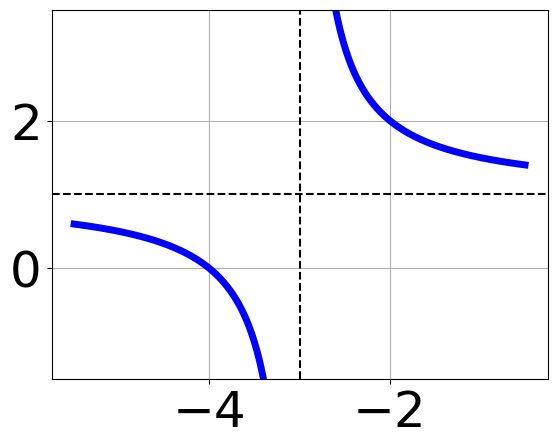
\includegraphics[width = 0.3\textwidth]{../Figures/rationalEquationToGraphDB.png}\end{multicols}\item None of the above.
\end{enumerate} }
\litem{
Solve the rational equation below. Then, choose the interval(s) that the solution(s) belongs to.\[ \frac{-4x}{2x -2} + \frac{-3x^{2}}{6x^{2} -6} = \frac{7}{3x + 3} \]\begin{enumerate}[label=\Alph*.]
\item \( x \in [-1.17,-0.51] \)
\item \( x_1 \in [-0.98, 1.34] \text{ and } x_2 \in [-8.16,-1.17] \)
\item \( x_1 \in [-0.98, 1.34] \text{ and } x_2 \in [1,6] \)
\item \( x \in [-3.3,-1.51] \)
\item \( \text{All solutions lead to invalid or complex values in the equation.} \)

\end{enumerate} }
\end{enumerate}

\end{document}